\chapter{Post-Exploitation}
\markboth{Post-Exploitation}{}

\section{Privilege Escalation}
Ora che è stato ottenuto l'accesso al sistema, il prossimo passo è quello di ottenere quanti più privilegi possibile.

\subsection{Fallimento delle strategie automatizzate}
Dal momento che la suite \emph{Metasploit} non ha dato i risultati sperati, ovviamente non è possibile utilizzare i moduli \emph{post} in quanto non è stato possibile generare una sessione. Quindi non potendo utilizzare questo strumento e non avendo trovato vulnerabilità del sistema nei report, si è deciso di continuare con l'analisi manuale
\subsection{Privilege Escalation orizzontale}
Dalla sessione \emph{SSH} dell'utente \textbf{mbrown}, un primo tentativo che è possibile effettuare è provare a cambiare utente sfruttando le password scoperte in precedenza. Utilizzando il comando \texttt{su} su entrambi gli utenti, il risultato è illustrato nella Figura \ref{fig:su}
\begin{figure}[h]
    \begin{subfigure}{0.5\textwidth}
        \hspace{0.15\textwidth}
        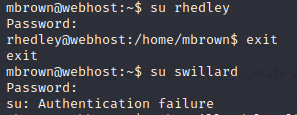
\includegraphics[width=0.6\textwidth]{capitoli/figure/su-users.png}
        \caption{Risultato cambio utente con \texttt{su}}
        \label{fig:su-users}
    \end{subfigure}
    \begin{subfigure}{0.5\textwidth}
        %\hspace{0.05\textwidth}
        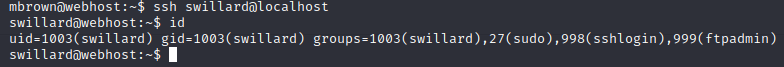
\includegraphics[width=1\textwidth]{capitoli/figure/su-users-ssh.png}
        \caption{Cambio utente con \emph{SSH}}
        \label{fig:su-users-ssh}
    \end{subfigure}
    \caption{Risultati cambio utente}
    \label{fig:su}
\end{figure}

Il cambio utente con \textbf{rhedley} ha successo (confermando anche l'esattezza della password) mentre con \textbf{swillard} non si ha successo (la password potrebbe non essere quella). Tuttavia un tentativo \emph{creativo} per provare a cambiare utente, come mostrato in Figura \ref{fig:su-users-ssh}, consiste nel provare a cambiare utente tramite \emph{SSH} e non solo questo tentativo ha successo, ma non richiede nemmeno la password dell'utente.\\
Per quanto riguarda \emph{FTP}, con l'utente \textbf{rhedley} si ha ancora una volta successo, mentre con l'utente \textbf{swillard}, di nuovo, non si ha successo.

\subsection{Scoperta di un backup}
Ritornando per un attimo alla shell di \textbf{mbrown}, dalle informazioni recuperate in precedenza sappiamo che esiste un \textbf{backup} sul server. Per cui quello che si può fare è cercare questo backup all'interno del filesystem. Per cercarlo si può usare il comando \texttt{find} grazie al quale possiamo effettuare una ricerca in tutto il filesystem. Immaginando che il nome del backup contenga proprio la parola \emph{backup}, si può lanciare il seguente comando:
\begin{lstlisting}[language=bash]
    find / backup 2>/dev/null | grep backup
\end{lstlisting}
dove con \texttt{2>/dev/null} si evita la stampa degli errori e con \texttt{grep} mostriamo a schermo solo i path che contengono effettivamente la parola \emph{backup}.

Una volta eseguito il comando, il risultato è il seguente:
\begin{figure}[h]
    \centering
    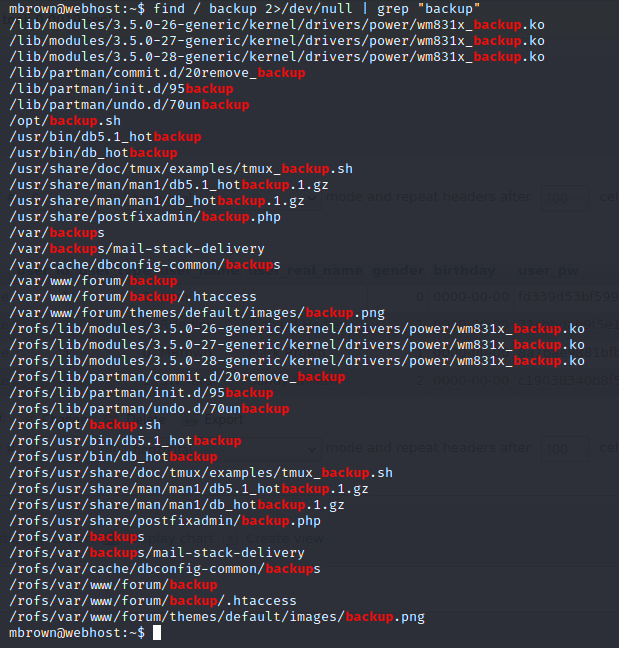
\includegraphics[width=0.4\textwidth]{capitoli/figure/find-backup.png}
    \caption{Output del comando \texttt{find}}
    \label{fig:find-backup}
\end{figure}

Dal risultato ottenuto salta subito all'occhio il percorso \textbf{\texttt{/opt/backup.sh}}, che potrebbe essere proprio lo script utilizzato per effettuare il backup.

\subsection{Decifratura del backup}
Provando a leggere il file come utente \textbf{mbrown} porta ad un \emph{permesso negato}, quindi è necessario cambiare utente nella speranza che l'altro abbia i permessi necessari. Con l'utente \textbf{rhedley} la lettura del file porta al seguente risultato:

\begin{figure}[h]
    \centering
    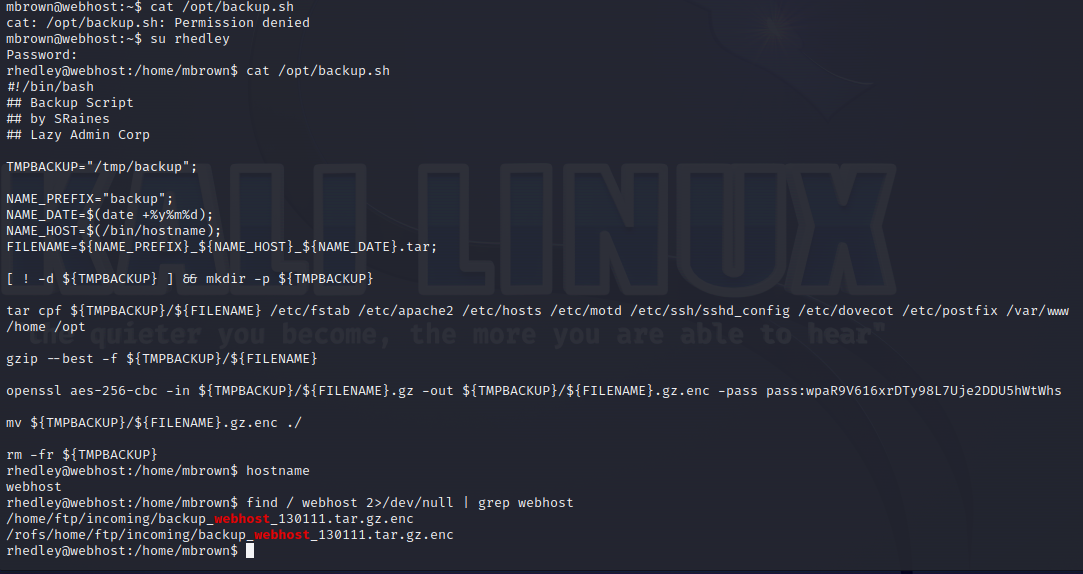
\includegraphics[width=0.7\textwidth]{capitoli/figure/backup-cat.png}
    \caption{Contenuto di \emph{backup.sh} e localizzazione del file di backup}
    \label{fig:backup-cat}
\end{figure}

Come si può notare, è proprio lo script utilizzato per effettuare il backup e, inoltre, questo è cifrato con una chiave che però è stata lasciata in chiaro proprio all'interno dello script. Ovviamente, lanciando lo stesso comando specificando l'opzione \texttt{-d} e il nome del backup, quello che succede è che decifriamo il backup. Una volta compreso il funzionamento dello script e il nome utilizzato per salvarlo, basta semplicemente specificare quello come nome di input (Figura \ref{fig:backup-cat}) e come nome di output si è scelto semplicemente \textbf{decrypted.tar.gz}. Quindi, il file ottenuto dalla decifratura è un archivio \texttt{.tar.gz} e, per evitare di lavorare direttamente sulla macchina, si effettua il login tramite \emph{FTP} con l'utente \textbf{rhedley} e si effettua il download del file che si trovava nel path \emph{ftp/incoming} (visto dallo script), come mostrato di seguito:
\begin{figure}[h]
    \centering
    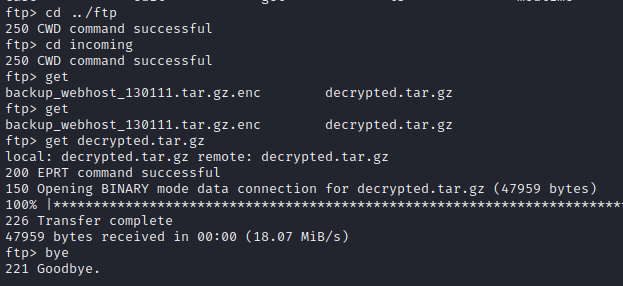
\includegraphics[width=0.7\textwidth]{capitoli/figure/ftp-rhedley-decrypted.png}
    \caption{Download del backup tramite \emph{FTP}}
    \label{fig:ftp-decrypted}
\end{figure}

Una volta effettuato il download, l'archivio viene estratto prima tramite \texttt{gzip} e successivamente tramite \texttt{tar}, come mostrato di seguito:
\begin{figure}[h]
    \begin{subfigure}{0.5\textwidth}
        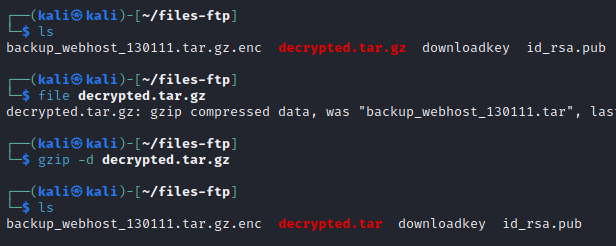
\includegraphics[width=1\textwidth]{capitoli/figure/decrypted-1.png}
        \caption{Estrazione con \texttt{gzip}}
        \label{fig:decrypted-1}
    \end{subfigure}
    \begin{subfigure}{0.5\textwidth}
        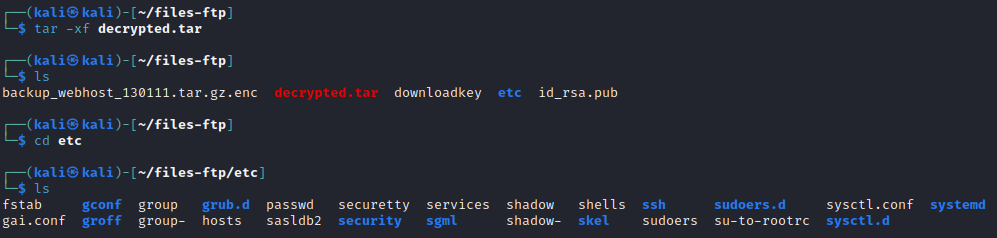
\includegraphics[width=1\textwidth]{capitoli/figure/decrypted-2.png}
        \caption{Estrazione con \texttt{tar} e visita del contenuto}
        \label{fig:decrypted-2}
    \end{subfigure}
    \caption{Estrazione e contenuto del backup}
    \label{fig:decrypted}
\end{figure}

Come si può vedere nella Figura \ref{fig:decrypted-2}, il contenuto del backup è il contenuto della cartella \emph{/etc} e, visualizzando il contenuto, si nota la presenza dei file \textbf{passwd} e \textbf{shadow}.

\subsection{Cracking delle password trovate all'interno del backup}
Utilizzando il tool \texttt{unshadow}, si possono ricostruire gli hash presenti all'interno dei due file e salvarli all'interno di un file che è stato chiamato \textbf{password}. Successivamente si può dare l'output di prima in pasto ad un tool di \emph{Offline Password Cracking} come \texttt{john}. Il risultato è mostrato di seguito:
\begin{figure}[h]
    \begin{subfigure}{0.5\textwidth}
        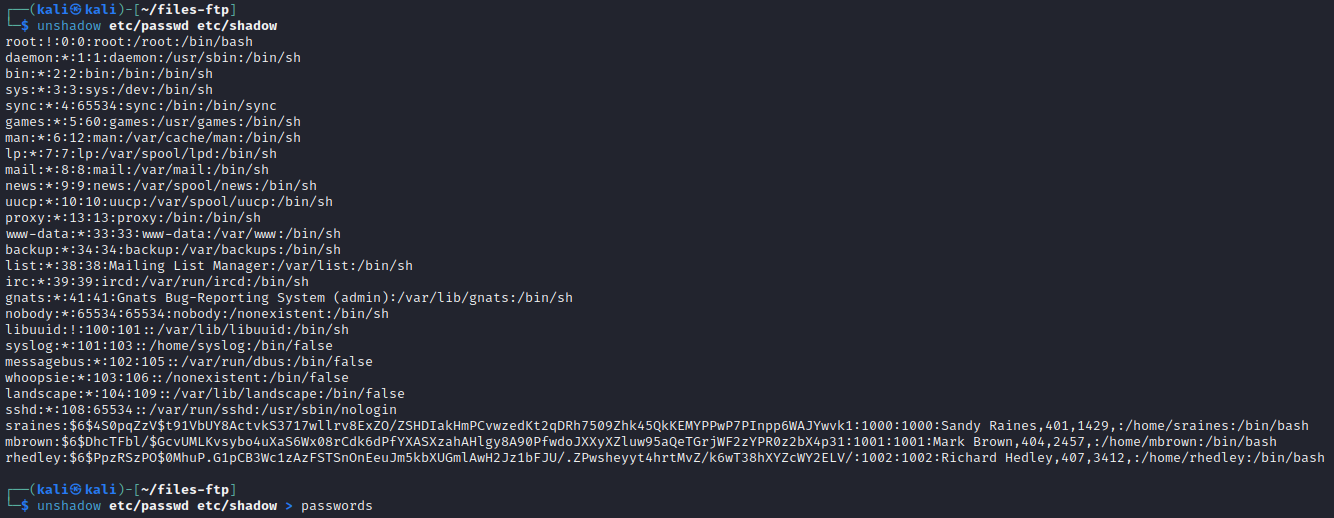
\includegraphics[width=1\textwidth]{capitoli/figure/unshadow.png}
        \caption{Ricostruzione degli hash delle password}
        \label{fig:unshadow}
    \end{subfigure}
    \begin{subfigure}{0.5\textwidth}
        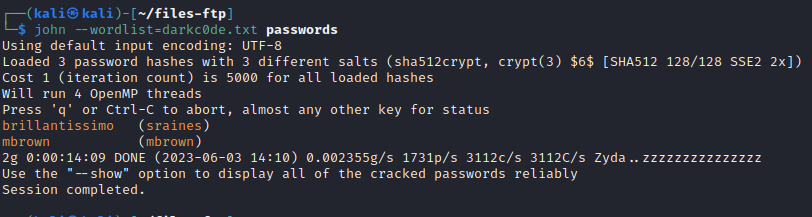
\includegraphics[width=1\textwidth]{capitoli/figure/passwd-john-recovered.png}
        \caption{Cracking delle password con \texttt{john}}
        \label{fig:john}
    \end{subfigure}
    \caption{Recupero della password di un nuovo utente}
    \label{fig:password-cracking}
\end{figure}

Per il cracking sono state utilizzate varie wordlist, ma l'unica che ha dato un risultato concreto è stata \textbf{darkc0de}.\\
A quanto sembra è stata recuperata sia la password di \textbf{mbrown} che di un nuovo utente chiamato \textbf{sraines}, tuttavia la password di \textbf{mbrown} non è quella recuperata e, inoltre, non esiste nessun utente \textbf{sraines}, come illustrato di seguito:

\begin{figure}[h]
    \centering
    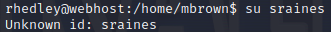
\includegraphics[width=0.5\textwidth]{capitoli/figure/sraines.png}
    \caption{Tentativo di cambio utente con \textbf{sraines}}
    \label{fig:sraines}
\end{figure}

\subsection{Privilege Escalation Verticale}
L'ultimo tentativo che si può fare è quello di tentare entrambe le password per gli unici due utenti di cui ancora non sappiamo la password: \textbf{mbrown} e \textbf{swillard}. Sorprendentemente, la password \textbf{brillantissimo} è proprio la password di \textbf{swillard} e, adesso, possiamo effettuare il login come quest'ultimo senza utilizzare l'approccio dell'\emph{SSH}. A questo punto, per capire il prossimo passo da eseguire bisogna capire quale sia la password dell'utente \textbf{root} o di un \textbf{sudoer}. Per visualizzare la lista dei \emph{sudoer} basta leggere il file \emph{/etc/groups} e vedere quali utenti hanno il gruppo \texttt{sudo}. L'output della lettura, effettuata utilizzando il filtro \texttt{grep} è il seguente:
\begin{figure}[h]
    \centering
    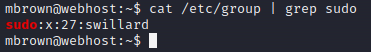
\includegraphics[width=0.5\textwidth]{capitoli/figure/sudo.png}
    \caption{Lista dei \emph{sudoer}}
    \label{fig:sudo}
\end{figure}

A quanto pare l'unico utente con i permessi di \texttt{sudo} è proprio \textbf{swillard}, di cui abbiamo appena scoperto la password. A questo punto, effettuando il login come quest'ultimo ed eseguendo il comando \texttt{sudo su} quello che si ottiene è che si diventa utente \textbf{root}, come mostrato di seguito:
\begin{figure}[h]
    \centering
    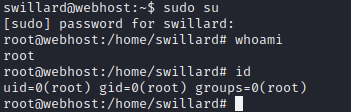
\includegraphics[width=0.6\textwidth]{capitoli/figure/root.png}
    \caption{Cambio ad utente \textbf{root}}
    \label{fig:root}
\end{figure}

Così facendo, è stato possibile effettuare una violazione completa del sistema assumendo pieno controllo sulla macchina.
\section{Maintaining Access}
Ora che la macchina è stata completamente violata, il prossimo passo da eseguire è l'installazione di una backdoor per ottenere immediamente i privilegi di utente \textbf{root}

\subsection{Creazione della backdoor}
Un'informazione molto importante che ci serve per creare una backdoor è l'architettura del processore della macchina target, in quanto ci sono payload differenti in base all'architettura della macchina target. Per mostrare l'architettura della macchina basta semplicemente eseguire il comando \texttt{arch}, come mostrato di seguito:
\begin{figure}[h]
    \centering
    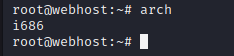
\includegraphics[width=0.3\textwidth]{capitoli/figure/arch.png}
    \caption{Architettura del sistema}
    \label{fig:arch}
\end{figure}

Come si può notare il sistema è eseguito su un processore \emph{Intel x86} a \textbf{32 bit}. Ora che è stata ottenuta quest'informazione, si può procedere con la generazione della backdoor. Per la creazione è stato usato \texttt{msfvenom}, un modulo della suite \emph{Metasploit} che si occupa proprio della generazione di backdoor. Si è deciso di generare una backdoor di tipo \emph{Reverse Shell} e per crearla basta lanciare \texttt{msfvenom} specificando architettura, sistema operativo e i parametri di connessione, come mostrato di seguito:
\begin{figure}[h]
    \centering
    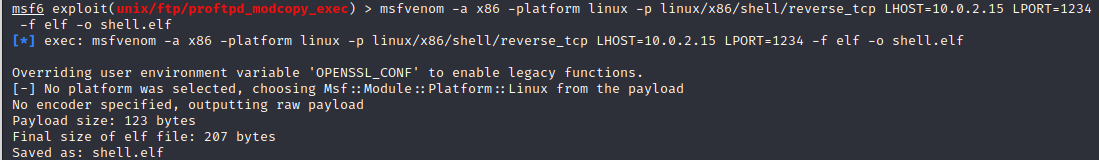
\includegraphics[width=0.7\textwidth]{capitoli/figure/backdoor-msfvenom.png}
    \caption{Creazione della backdoor con \texttt{msfvenom}}
    \label{fig:backdoor-msfvenom}
\end{figure}

In seguito all'esecuzione del modulo, viene generato un file chiamato \textbf{shell.elf} (il nome che è stato specificato) che sarà prorpio il payload da avviare sulla macchina target.

\subsection{Trasferimento della backdoor sull'asset}
Ora che è stato generato il payload, bisogna trasferirlo sull'asset. Per farlo è stato utlizzato il web server \emph{Apache} preconfigurato su \textbf{Kali}. Infatti basta semplicemente spostare il payload nella cartella del web server e avviarlo, come mostrato di seguito:
\begin{figure}[h]
    \centering
    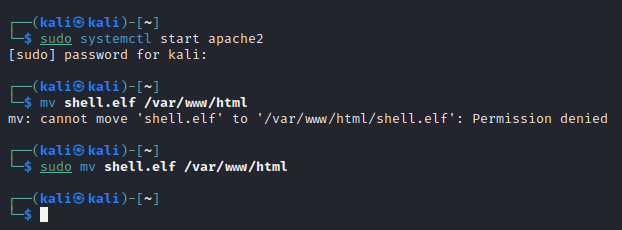
\includegraphics[width=0.5\textwidth]{capitoli/figure/backdoor-apache.png}
    \caption{Caricamento del payload sul web server}
    \label{fig:backdoor-apache}
\end{figure}

Ora che il payload è caricato sul web server, basta accedere sulla macchina target e, tramite lo strumento \texttt{wget} specificare l'indirizzo di \textbf{Kali} e il file che si vuole ottenere, come mostrato di seguito:
\begin{figure}[h]
    \centering
    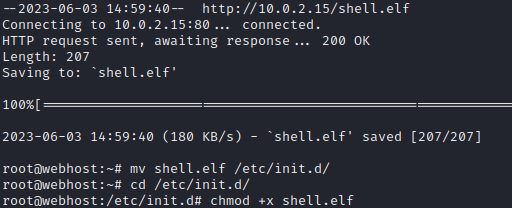
\includegraphics[width=0.5\textwidth]{capitoli/figure/backdoor-transfer.png}
    \caption{Trasferimento del payload sull'asset}
    \label{fig:backdoor-transfer}
\end{figure}

Una volta scaricato, per permettere l'esecuzione all'avvio del payload (e anche per renderlo meno visibile) bisogna spostarlo nella cartella \emph{init.d} che contiene tutti i file che devono essere eseguiti all'avvio e, una volta lì, abilitare i permessi di esecuzione altrimenti (ovviamente) non può essere eseguito.

\subsection{Abilitazione della backdoor}
Per poter eseguire la backdoor basta semplicemente avviare l'eseguibile, tuttavia, non è quello che ci aspettiamo da un utente ad ogni avvio. Per cui bisogna scrivere un exploit che si occuperà di avviare in automatico il payload e fare in modo che questo venga eseguito all'avvio del sistema. L'exploit sarà un semplicissimo script chiamato \emph{in.sh} che semplicemente avvierà il payload, come mostrato di seguito:
\begin{figure}[h]
    \centering
    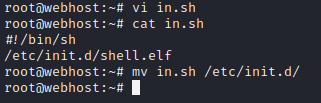
\includegraphics[width=0.5\textwidth]{capitoli/figure/backdoor-script.png}
    \caption{Scrittura dell'exploit}
    \label{fig:backdoor-script}
\end{figure}

Ovviamente, anch'esso sarà posizionato nella cartella \emph{init.d} insieme agli altri file da eseguire all'avvio. Essendo che il sistema è \emph{pre-systemd}, per fare in modo che un file venga eseguito all'avvio bisogna manipolare il file \emph{rc.local} e, per farlo, basta lanciare i seguenti comandi:
\begin{lstlisting}[language=bash]
    sed -i '\$d' /etc/rc.local
    echo "sh /etc/init.d/in.sh" >> /etc/rc.local
    echo "exit 0" >> /etc/rc.local
\end{lstlisting}

Così facendo il file \emph{in.sh} sarà eseguito in automatico ad ogni avvio e comincierà a contattare la macchina \textbf{Kali} sulla porta 1234 fin quando questa non si metterà in ascolto.

\subsection{Impossibilità di testing della backdoor}
Essendo che l'asset analizzato è una macchina virtuale realizzata con lo scopo di essere una sfida \emph{CTF}, per evitare che in seguito ad operazioni di manipolazione del sistema ci si trovi in una situazione irrecuperabile (la cui unica soluzione sia riscaricare e reinstallare la macchina) il sistema è \emph{live}, ovvero ogni modifica fatta rimane solo in \emph{RAM} e non viene alterato in alcun modo. Questo, tuttavia, significa che non si può testare il corretto funzionamento della backdoor all'avvio in quanto un riavvio del sistema comporta la cancellazione di ogni modifica effettuata e quindi anche del payload e dello script, nonchè del file \emph{rc.local} modificato. Ad ogni modo, eseguendo manualmente l'exploit e avviando l'handler di \emph{Metasploit} il risultato è il seguente:
\begin{figure}[h]
    \centering
    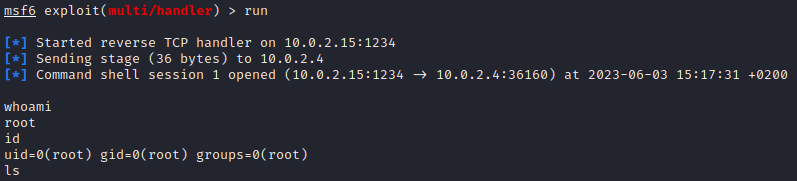
\includegraphics[width=0.7\textwidth]{capitoli/figure/metasploit-backdoor.png}
    \caption{Utilizzo della backdoor}
    \label{fig:backdoor-metasploit}
\end{figure}

Quindi come si può vedere l'exploit funziona correttamente (ed è anche possibile eseguire l'upgrade ad una sessione meterpreter come mostrato in Figura \ref{fig:backdoor-meterpreter}) se avviato manualmente quindi, al netto di errori nei comandi lanciati per manipolare \emph{rc.local}, è lecito supporre che la backdoor sia stata installata correnttamente e che venga avviata ad ogni riavvio del sistema.

\begin{figure}[h]
    \centering
    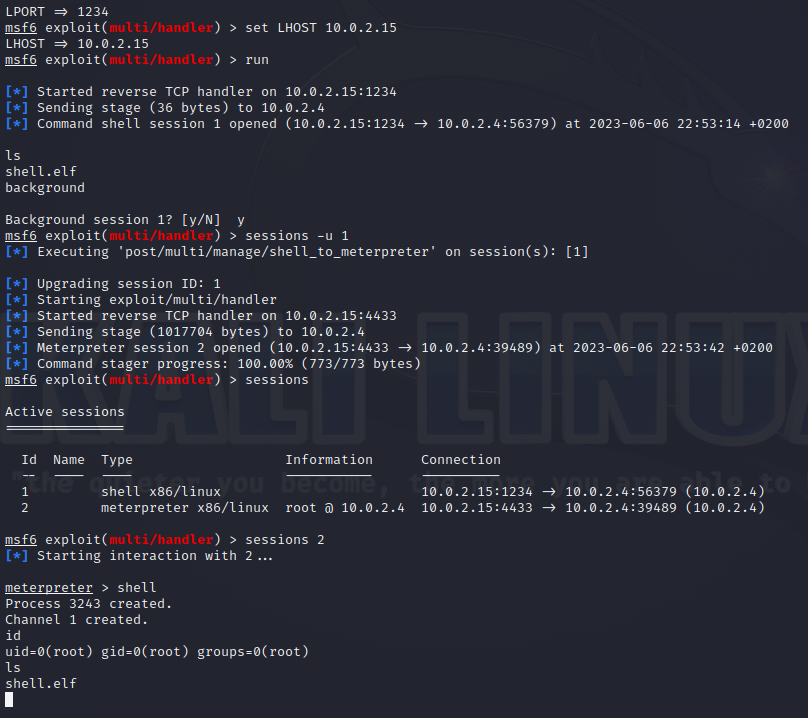
\includegraphics[width=0.4\textwidth]{capitoli/figure/backdoor-metrpreter.png}
    \caption{Upgrade a sessione \emph{Meterpreter}}
    \label{fig:backdoor-meterpreter}
\end{figure}
